\documentclass{beamer}
\usetheme{Boadilla}
\usecolortheme{seahorse}
\setbeamercolor{palette primary}{bg=blue!15,fg=blue!80!black}
\usepackage[utf8]{inputenc}
\usepackage{graphicx}

\title{QML (Angle Embedding) y DNN para b-Tagging en Jets de bajo momento}
\author{Juan}
\institute{Instituto de Física}
\date{12 de agosto de 2025}

\begin{document}

\begin{frame}
  \titlepage
\end{frame}

\begin{frame}{Agenda}
  \tableofcontents
\end{frame}

\section{Introducción}
\begin{frame}{Contexto y Objetivo}
  \begin{itemize}
    \item Que son los jets?
    % vamos a mostrar dos imagenes horizontalmente
    \begin{figure}
      \centering
      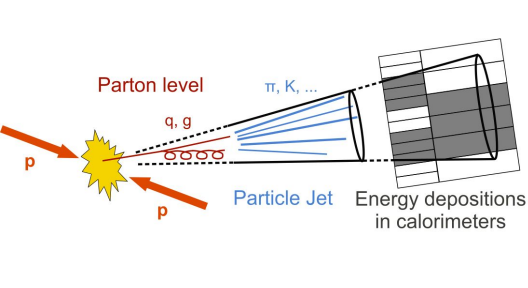
\includegraphics[width=0.45\textwidth]{jet1.png}
      \hfill
      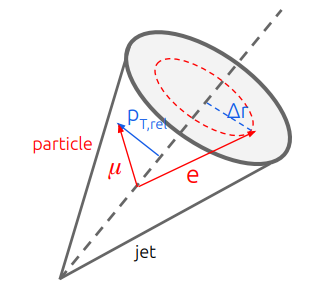
\includegraphics[width=0.45\textwidth]{jet2.png}
    \end{figure}
  \end{itemize}
\end{frame}

\begin{frame}{Contexto y Objetivo}
  \begin{itemize}
    \item Jets de bajo momento (LowPt) en colisiones pp.
    % vamos a mostrar tres imagenes dos verticalmente y una horzontal
    \begin{figure}
      \centering
      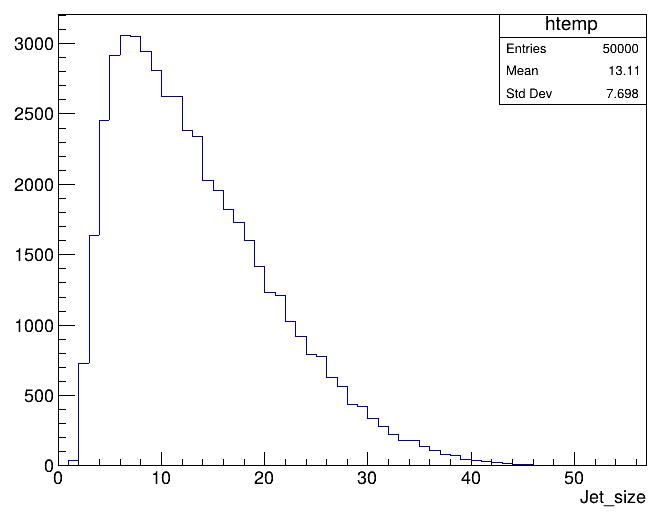
\includegraphics[width=0.4\textwidth]{njetl.png}
      \hfill
      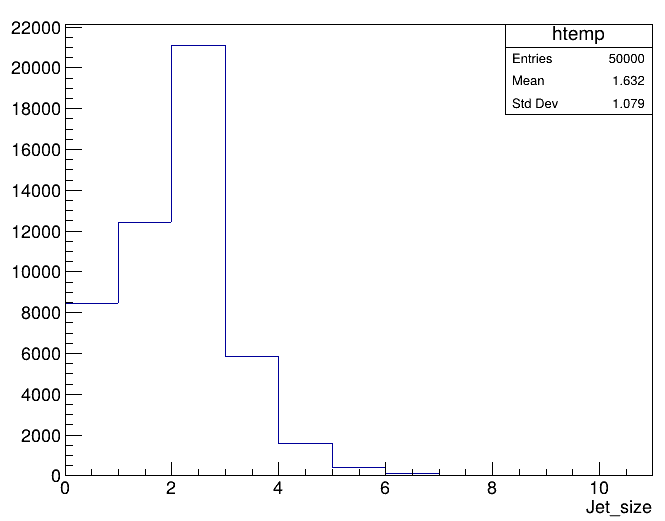
\includegraphics[width=0.4\textwidth]{njeth.png}
      \hfill
      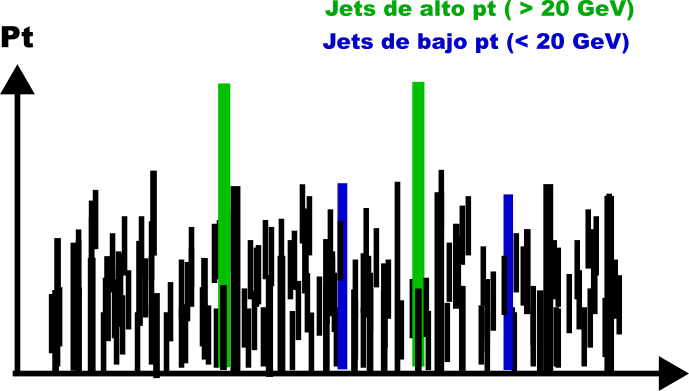
\includegraphics[width=0.4\textwidth]{lowpt.png}
    \end{figure}
  \end{itemize}
\end{frame}

\begin{frame}{Contexto y Objetivo}
  \begin{itemize}
    \item Motivante
    \begin{figure}
      \centering
      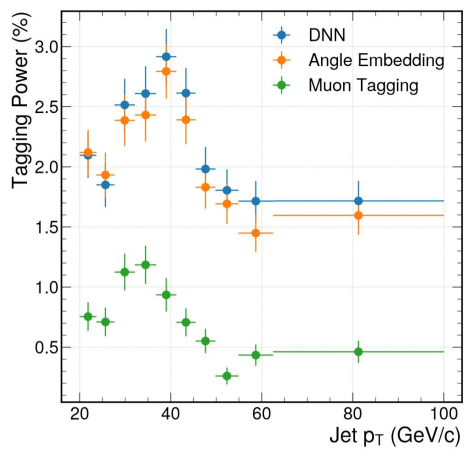
\includegraphics[width=0.45\textwidth]{motiv.png}
    \end{figure}
  \end{itemize}
\end{frame}

\begin{frame}
    \begin{figure}
    \centering
    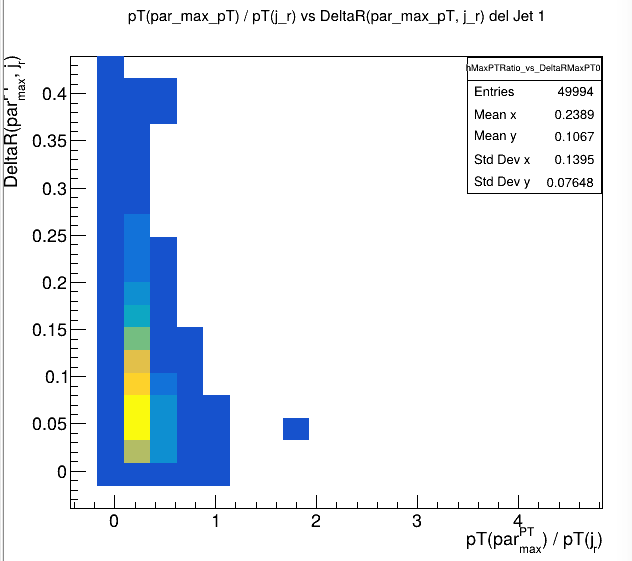
\includegraphics[width=0.47\textwidth]{lowptjet.png}
    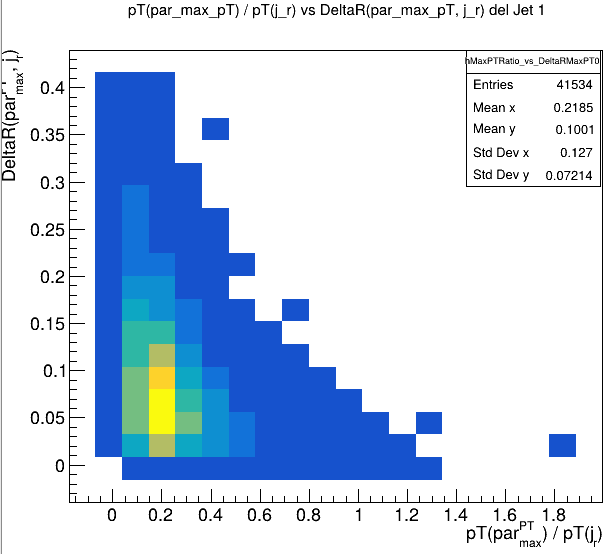
\includegraphics[width=0.47\textwidth]{higptjet.png}
  \end{figure}
\end{frame}

\section{Quantum Machine Learning}
\begin{frame}{¿Qué es QML?}
  \begin{itemize}
    \item Híbrido cuántico–clásico
    \item Se aprovecha superposición y entrelazamiento.
    \item Embedding de datos clásicos en qubits.
  \end{itemize}
\end{frame}

\begin{frame}{Angle Embedding}
  \begin{itemize}
    \item Para un vector $\mathbf{x}=[x_1,\dots,x_n]$ normalizado en $[-\pi,\pi]$.
    \item Aplica rotaciones $RX(x_i)$ o $RY(x_i)$ en cada qubit.
    \item n caracteristicas → n qubits.
  \end{itemize}
  \vspace{1em}
  \begin{figure}
    \centering
    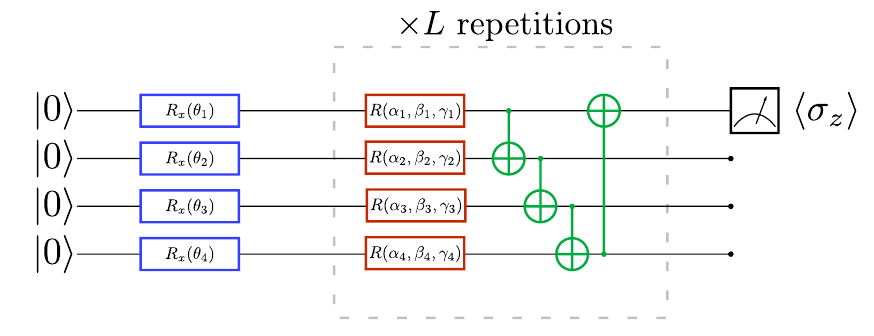
\includegraphics[width=0.6\textwidth]{angleemb.png}
  \end{figure}
\end{frame}

% una nueva diapositva unicamente para mostrar en pantalla completa una imagen
\begin{frame}{Angle Embedding}
  \begin{figure}
    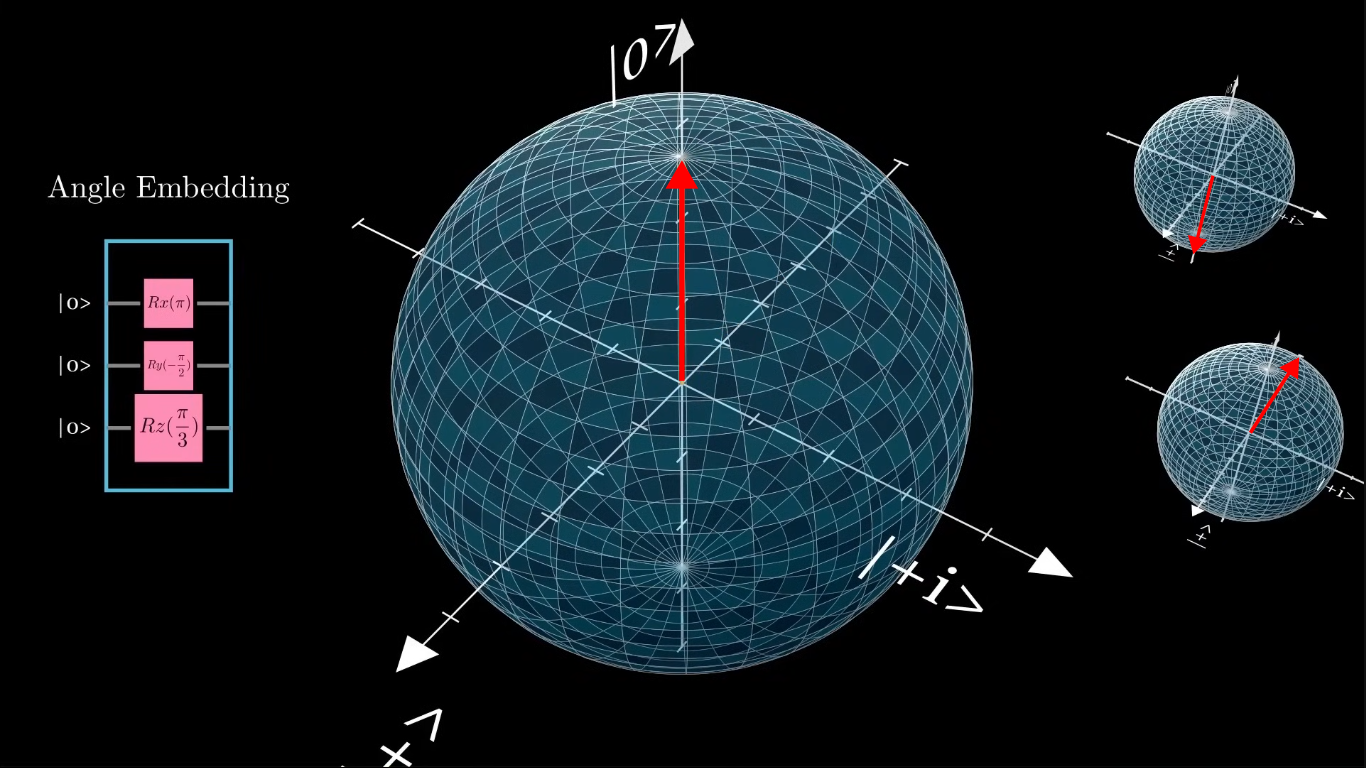
\includegraphics[width=1\textwidth]{blochh.png}
  \end{figure}
\end{frame}


\section{Circuito QML}
\begin{frame}{Detalles del Circuito}
  \begin{itemize}
    \item Dispositivo: \texttt{lightning.gpu}
    \item Embedding: \texttt{qml.AngleEmbedding(inputs, wires=0..15)}
    \item Capas: \texttt{qml.StronglyEntanglingLayers(weights, wires=0..15)}
    \item Salida: $\langle Z_0\rangle \in [-1,1]$
  \end{itemize}
  \vspace{1em}
  \begin{figure}
    \centering
    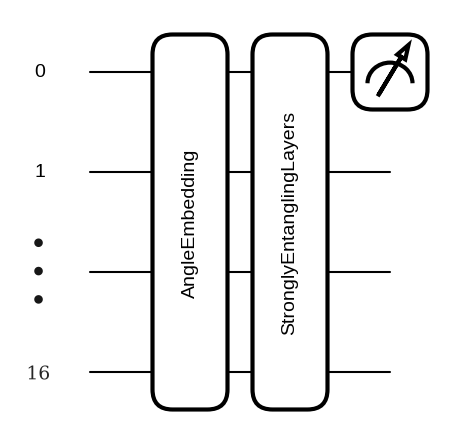
\includegraphics[width=0.4\textwidth]{circuito.png}
  \end{figure}
\end{frame}


\begin{frame}{StronglyEntanglingLayers: Correlaciones Cuánticas}
  \textbf{Cada capa contiene:}
  \begin{enumerate}
    \item \textbf{Rotaciones locales:} $RX(\theta)$, $RY(\phi)$, $RZ(\lambda)$ 
    \begin{itemize}
      \item Parámetros entrenables
      \item Orientan cada qubit individualmente
    \end{itemize}
    
    \item \textbf{Puertas entrelazantes:} CNOT, CZ
    \begin{itemize}
      \item Conectan qubits → correlaciones no-clásicas
      \item Estado global $\neq$ suma de estados individuales
    \end{itemize}
  \end{enumerate}

\end{frame}

\section{Metodología}
\begin{frame}{Flujo de Trabajo}
  \begin{enumerate}
    \item Carga y preprocesamiento de histogramas ROOT
    \item Normalización (arctan)
    \item \textbf{QML}: 16 qubits, \texttt{AngleEmbedding}, 4 capas de \texttt{StronglyEntanglingLayers}, medida \texttt{PauliZ}
    \item \textbf{DNN}: arquitectura 16-64-32-1 con ReLU/tanh
    \item Entrenamiento (Adam, 10 epochs, batch=64)
    \item Evaluación: AUC y Tagging Power
  \end{enumerate}
\end{frame}

\section{Resultados}
\begin{frame}{Métricas Comparativas}
  \begin{itemize}
    \item AUC y Tagging Power para cada dataset:
      \begin{itemize}
        \item Zbb\_LowPT, Zbb\_HighPT, Zp\_M30\_LowPT, Zp\_M100\_LowPT
      \end{itemize}
    \item Gráficas de:
      \begin{itemize}
        \item Distribución de predicciones
        \item Evolución de pérdida y accuracy
      \end{itemize}
  \end{itemize}
  \vspace{1em}
  \begin{figure}
    \centering
    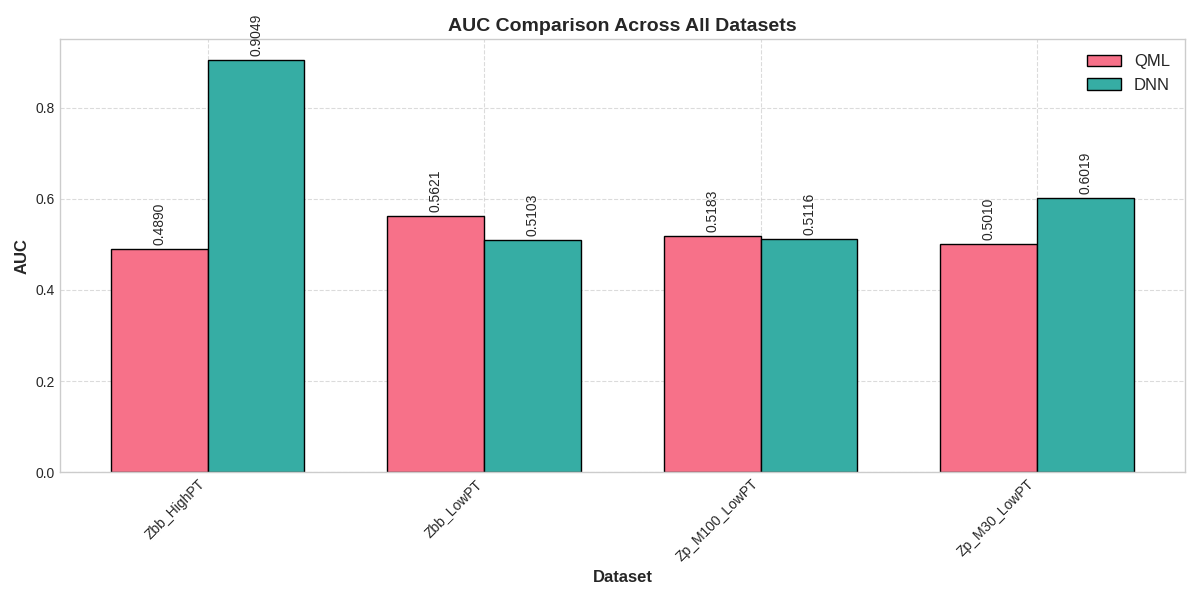
\includegraphics[width=0.75\textwidth]{resumen_hmmm/auc_all_datasets.png}
  \end{figure}
\end{frame}

\begin{frame}
  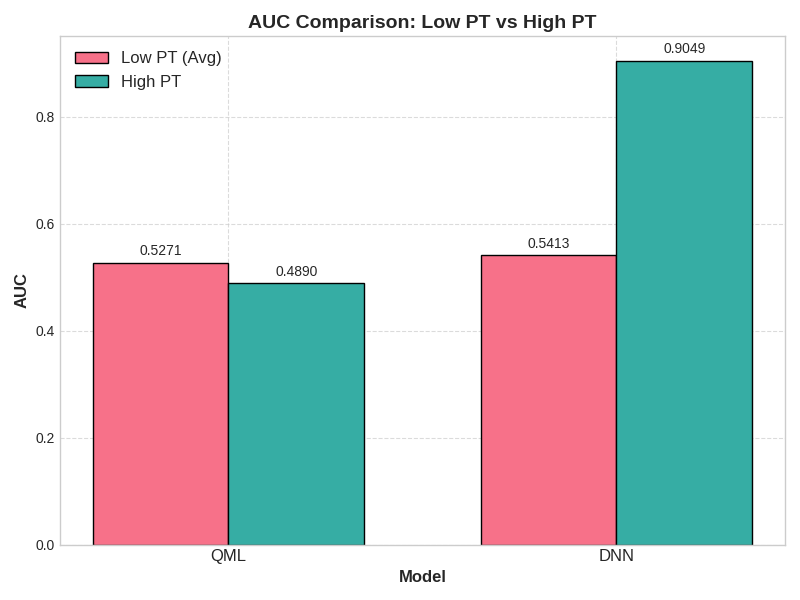
\includegraphics[width=1\textwidth]{resumen_hmmm/auc_low_vs_high_pt.png}
\end{frame}

\begin{frame}
  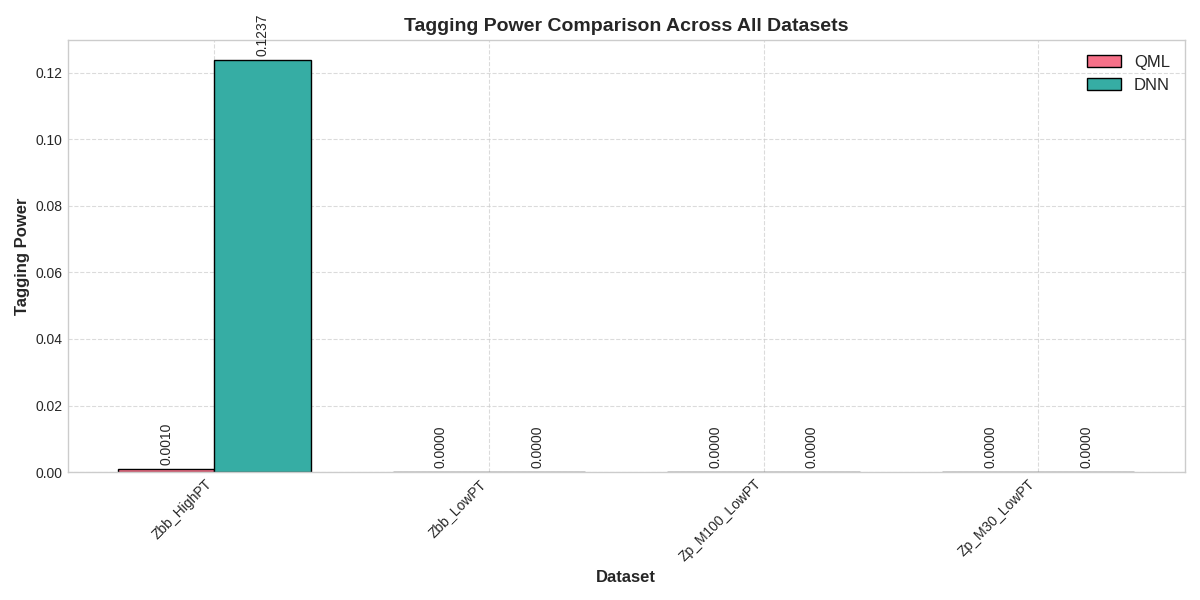
\includegraphics[width=1\textwidth]{resumen_hmmm/tagging_power_all_datasets.png}
\end{frame}

\section{Conclusiones}

\begin{frame}{Principales Conclusiones: Rendimiento}
  \begin{itemize}
    \item DNN vs QML: DNN mejor AUC (0.63 vs 0.52) y tagging en HighPT ($\epsilon \approx$0.12); QML casi no etiqueta.
    \item HighPT $<$ LowPT: DNN AUC~0.9 vs AUC~0.5; LowPt difícil de separar.
    \item Z normal $<$ Z': las muestras con masas teóricas distorsionan la distribución y reducen la discriminación.
  \end{itemize}
\end{frame}

\begin{frame}{Principales Conclusiones: Limitaciones y Siguientes Pasos}
  \begin{itemize}
    \item Muestra pequeña (1000 eventos)
    \item Explorar configuraciones distintas del cicuito.
    \item Explorar otras caracteristicas relevantes del jet.
  \end{itemize}
\end{frame}

\section{Referencias}

\begin{frame}
  \begin{thebibliography}{9}
    \bibitem{Exposicion}
      A. Gianelle et al., "First implementation of Quantum Machine Learning for b-jet tagging at LHCb", 2021. \href{https://indico.cern.ch/event/1053287/contributions/4442055/attachments/2332563/3975381/qml@lhcb_zuliani.pdf}{Link}
    \bibitem{angle_embedding}
      A. Gianelle et al., "Quantum Machine Learning for b-jet charge identification", 2022. \href{https://arxiv.org/pdf/2202.13943}{Link}
    \bibitem{Representacion en esfera de blochh}
      Youtube chanel 'Blochh Sphere', "Quantum Neural Networks explained", 2024.
    \end{thebibliography} \href{https://youtu.be/xL383DseSpE}{Video}
\end{frame}

\end{document}